% include the figures path relative to the master file
\graphicspath{{./content/intro/figures/}}

\section{Polarized cues used for attitude estimation}
\label{sec:pcues}

Polarized cues used for attitude estimation are based on three main concepts
which are presented in this section: (i) the Rayleigh scattering model and its
implications on the polarization by scattering, (ii) the polarization
parameters in pixel frame and its relation to camera, and (iii) the connection
between the polarized parameters in the pixel frame and the parameters used to
estimate the vehicle attitude.

% To understand the polarized cues that are used for attitude estimation, three
% main concepts are covered in this section: (i) the Rayleigh scattering model and
% interesting aspects of polarization by scattering, (ii) the polarization
% parameters in pixel frame and its relation to camera, and (iii) the
% relationship between the polarized parameters in the pixel frame and other
% parameters for attitude estimation.
% solar zenith: angle between the zenith and the center of the sun disk $\theta_s$
% solar elevation: altitude of the sun, angle between the horizon and the
% center of the sun disk $\alpha_s$
% solar azimuth: direction of the sun $\phi_s$, while $\theta_s, \alpha_s$
% define how high is the sun
% scattering angle $\lambda$: angular distance between the observed celestial
% point and the sun
% solar meridian: plane containing the sun and the observer
% Scattering plane: plane of observer,  celestial point observed and the sun
% Rayleigh model- direction of polarization is perpendicular to the scattering
% plane

\subsection{Rayleigh scattering model}
\label{subsec:rayleigh}
The unpolarized sunlight passing through our atmosphere gets scattered by
different particles within the atmosphere. Besides deviating the direction of
a propagated wave, this transition also changes the polarization state of the
incident light which can be explained using the Rayleigh scattering model.
Rayleigh scattering describes the scattering of light (or any
electromagnetic waves) by particles much smaller than their transmission
wavelength. Accordingly, it assumes that scattering particles of the atmosphere
are homogeneous and smaller than the wavelength of the sunlight. Despite these
assumptions, this model proved to be sufficient for describing skylight
scattering and polarization
patterns~\cite{pomozi2001clearsky,horvath2002ground}.

The Rayleigh model predicts that the unpolarized sunlight becomes linearly
polarized after being scattered by the atmosphere. Based on this model, two
main outcomes are drawn. On the one hand, \gls{dopl} is directly linked to the
scattering angle $\gamma$ according to:

\begin{equation}
  \label{eq:3}
  \rho_{l} = \rho_{l_{max}}\frac{1 - \cos^{2}(\gamma)}{1 + \cos^{
      2}(\gamma)}
\end{equation}

\noindent where $\rho_{l_{max}}$ is a constant equal to 1 in theory but
slightly less than 1 in practice due to some atmospheric
disturbances~\cite{pomozi2001clearsky}. The scattering angle $\gamma$ is
defined by the angle between the observed celestial vector $\vec{c}$ and the
sun vector $\vec{s}$ as presented in Fig.\,\ref{fig:scattering}. Note that
\gls{dopl} is 0 in the sun direction and maximum when the scattering angle is
$\frac{\pi}{2}$~\cite{smith2007polarization,miyazaki09sunlightpolarization}.

On the other hand, the scattered light is considered to be polarized and
orthogonal to the scattering plane.  Consequently, the Angle of Polarization is
directly related to the orientation of the scattering plane.

\begin{figure}
  \centering
  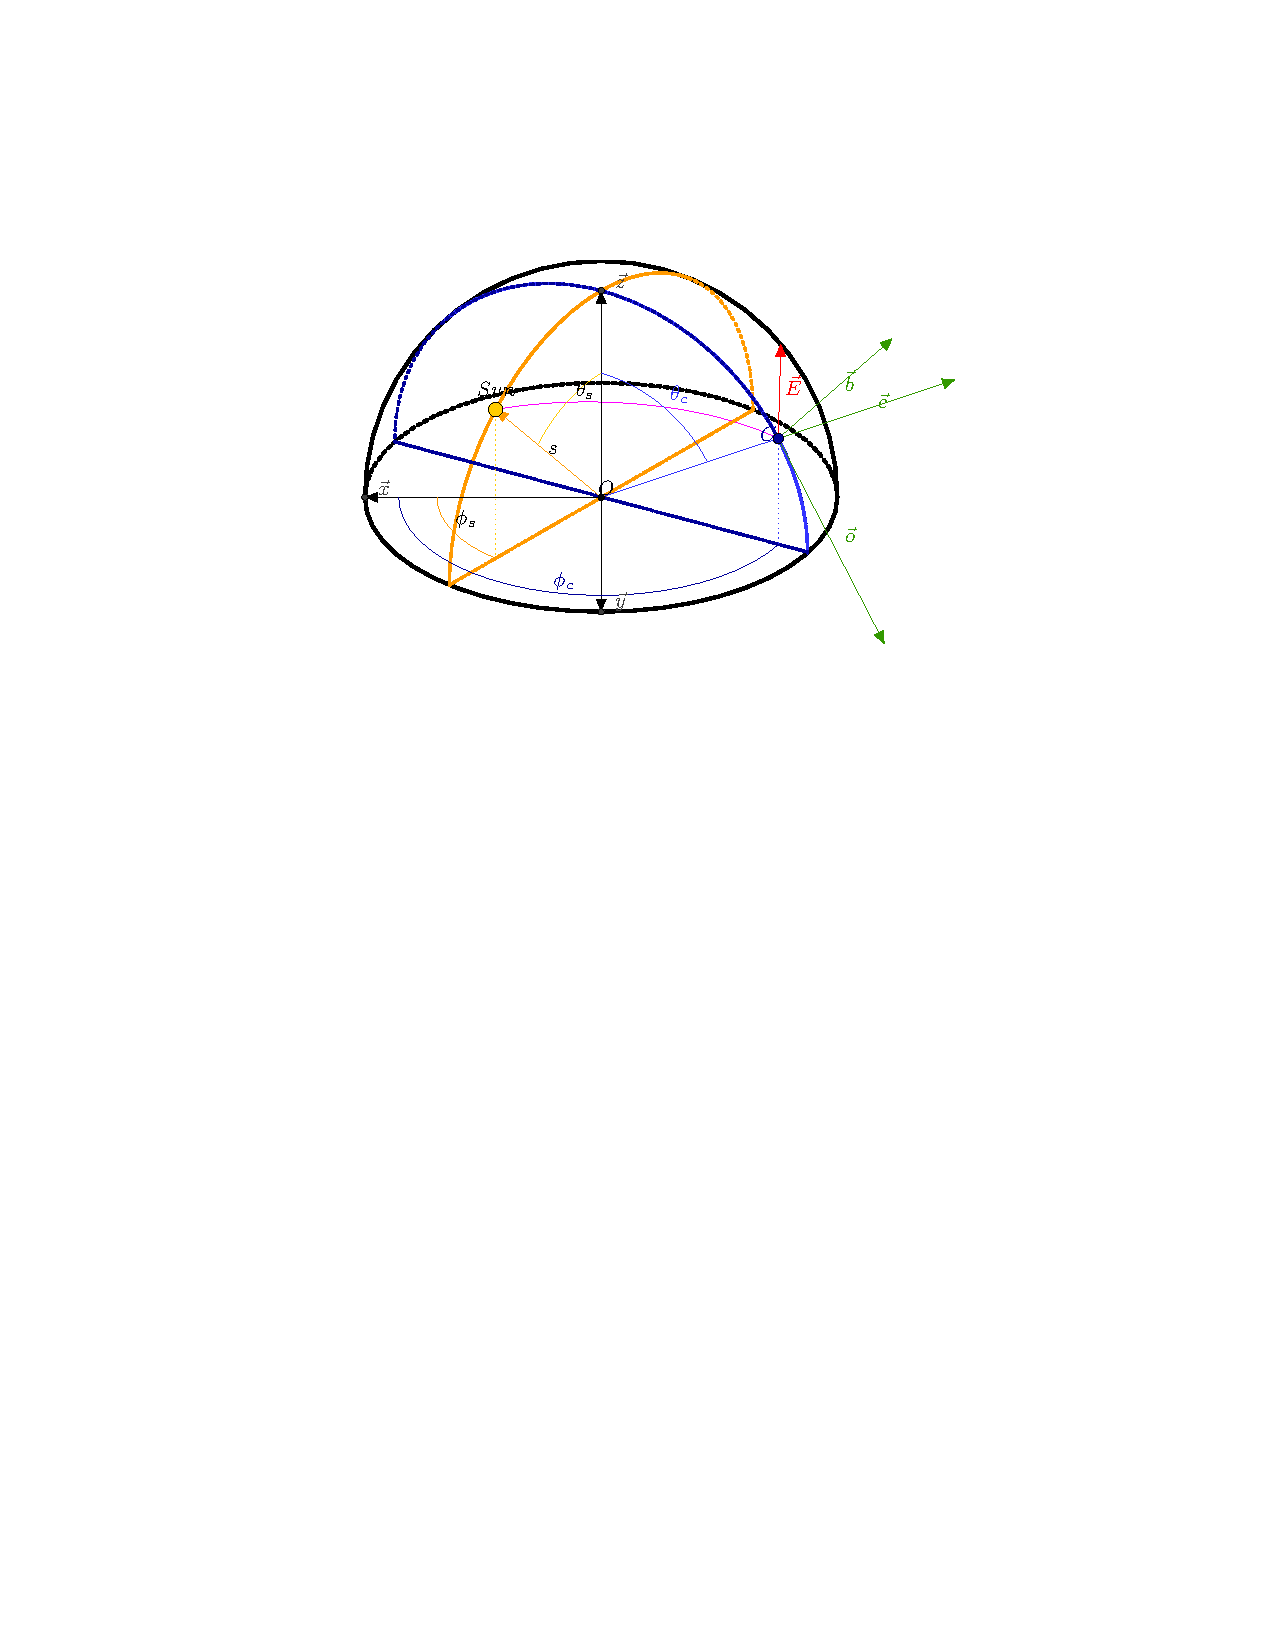
\includegraphics[width=0.47\textwidth]{./content/intro/figures/polasky-iros.pdf}
  \caption{Skylight polarization by scattering. Scattering plane is highlighted
  by light shade of red. ($\theta_s$, $\phi_s$) and ($\theta_c$, $\phi_c$)
  define the zenith and azimuth angle of sun and celestial point
  respectively. $\widehat{obc}$ defines the pixel frame, $\mathcal{P}$, and
  $\vec{E}$ is the electrical field orthogonal to the scattering plane.}
    \label{fig:scattering}
\end{figure}


\subsection{Polarization by scattering model in pixel frame}
\label{subsec:pscattering}
As presented Fig.\,\ref{fig:pixelframe}, an image is considered as a collection
of pixels and each pixel measures the polarization parameters of the light
traveling along a ray associated with that pixel. The pixel frame
$\mathcal{P}$ is defined accordingly with the ray which coincides with
$\vec{c}$. The camera calibration determines the relationship between pixels
and these 3D rays.

\begin{figure}
  \centering
  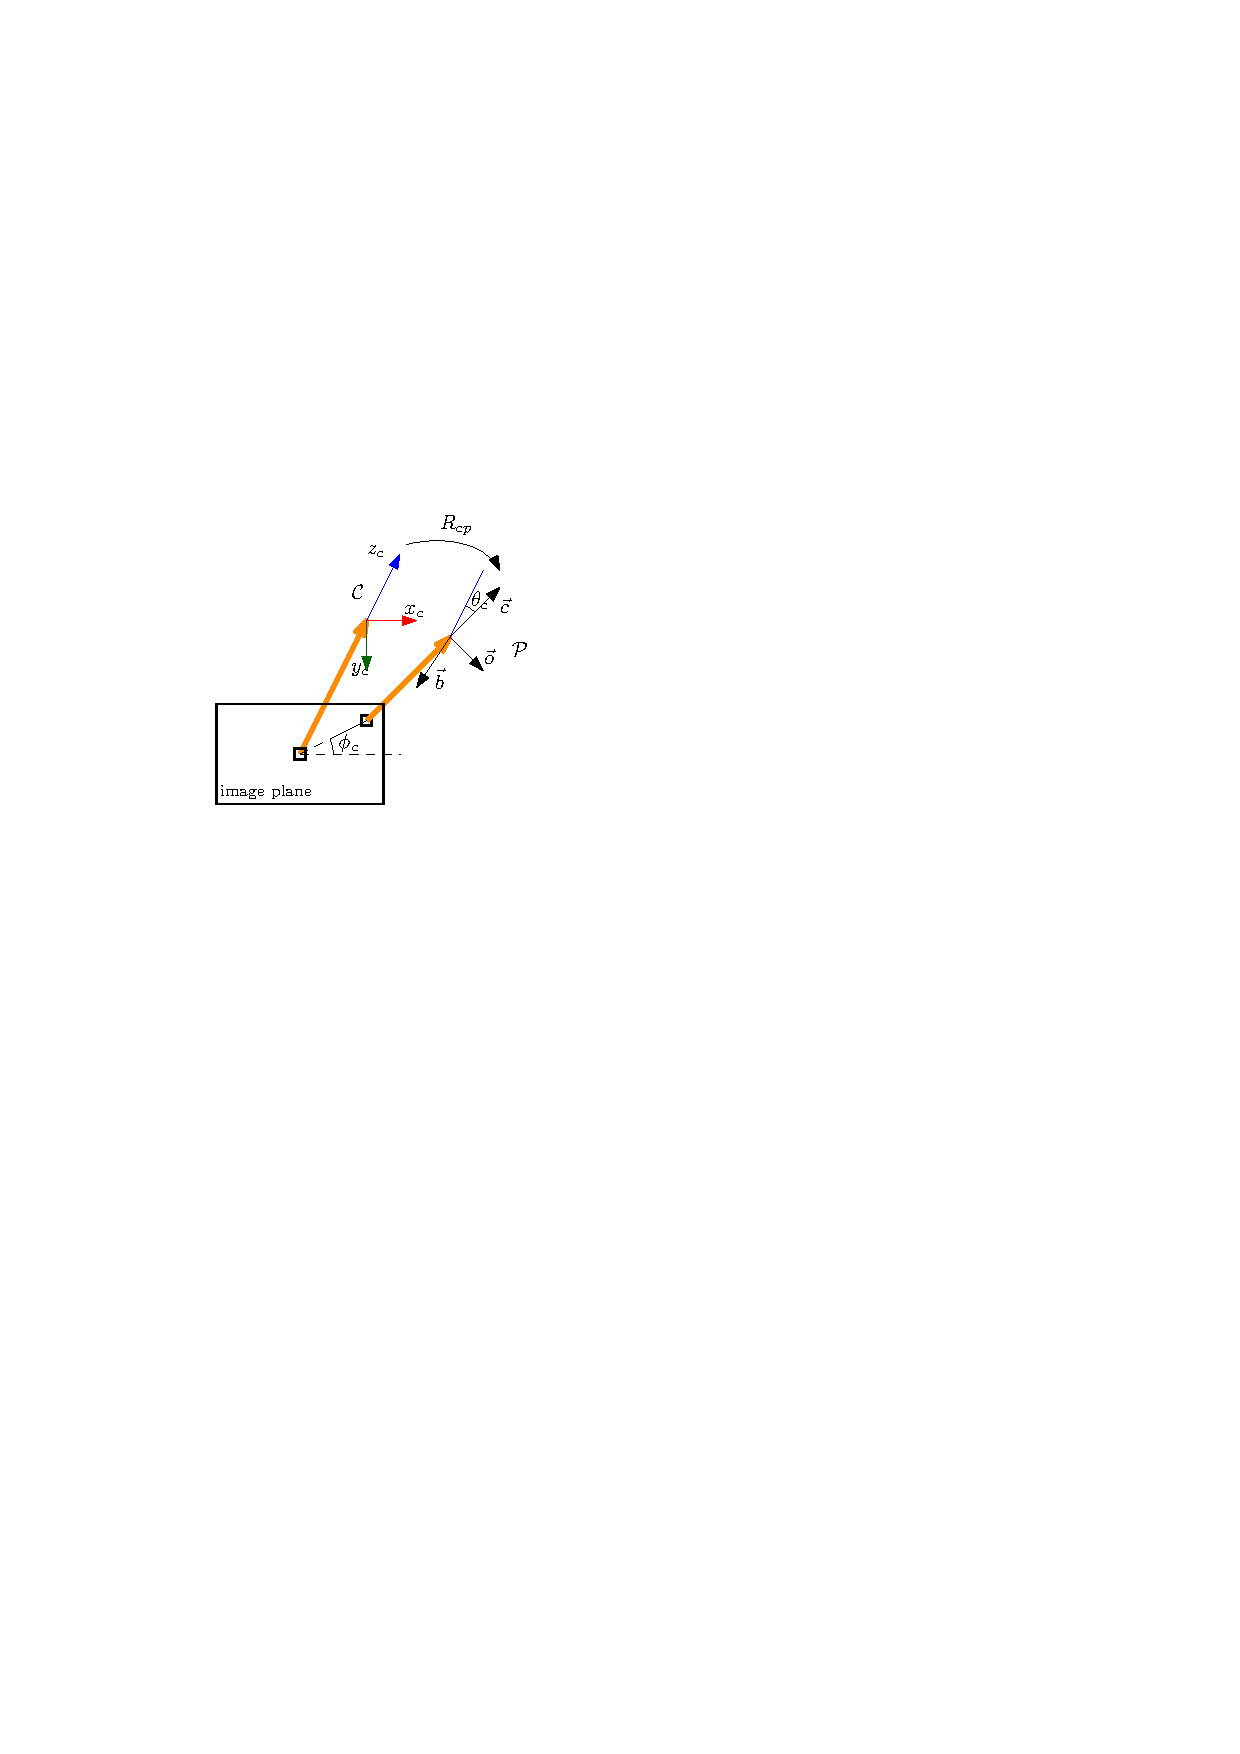
\includegraphics[scale=0.8]{./content/intro/figures/pixelframe.pdf}
  \caption{Rotation between the camera frame $\mathcal{C}$ and one pixel of the frame $\mathcal{P}$. The light ray associated to the pixels are represented in dark orange. The pixel that corresponds to the center of the image has obiously the same frame as the camera.}
    \label{fig:pixelframe}
\end{figure}

Let consider one pixel of the image with its associated pixel frame $\mathcal{P}$ ($\widehat{obc}$).
Based on Rayleigh scattering, the electric field of incident light after
scattering is perpendicular to the scattering plane that is defined by the
observer, celestial point, and the sun.
Accordingly, the normalized electric field vector $\vec{E}$ in the world frame
is presented as the normalized cross product of $\vec{s}$ and
$\vec{c}$ as shown in Eq.\,\eqref{Eq:E}.

\begin{equation}
\vec{E}=\frac{\vec{s}\wedge \vec{c}}{\left\Vert \vec{s}\wedge
    \vec{c}\right\Vert }
\label{Eq:E}
\end{equation}

The same measurement in the pixel frame $\mathcal{P}$ is represented as:
% However measuring the skylight polarization pattern and \gls{aop}, the electric
% field in the pixel frame $\mathcal{P}$ ($\widehat{obc}$) is represented as:

\begin{equation}
E_{obc}=\left[\begin{array}{c}
E_{o}\\
E_{b}\\
0
\end{array}\right]=\left[\begin{array}{c}
\cos\alpha\\
\sin\alpha\\
0
\end{array}\right]
\label{Eq:Eproj}
\end{equation}
\noindent where $\alpha$ is the measured \gls{aop} associated to the corresponding pixel.
Combining Eq.\,\eqref{Eq:E}~\&~\eqref{Eq:Eproj} and using the
scattering angle $\gamma$, between $\vec{s}$ and $\vec{c}$ lead to:
\begin{equation}
  \begin{cases}
(s\wedge c)\cdot o & =\sin\gamma\cos\alpha\\
(s\wedge c)\cdot b & =\sin\gamma\sin\alpha
\end{cases}
\label{eq:E0EB vect-1-1}
\end{equation}

Applying the vector triplet cross product rule on Eq.\,\eqref{eq:E0EB
  vect-1-1} results in:
\begin{equation}
\begin{cases}
s\cdot b & =\sin\gamma\cos\alpha\\
s\cdot o & =-\sin\gamma\sin\alpha
\end{cases}
\label{eq:scal-b-o}
\end{equation}
Using Eq.\,\eqref{eq:3}, the scattering angle $\gamma$ is expressed as:
\begin{equation}
\cos\gamma=s\cdot c=\pm\sqrt{\frac{1-\rho_{l}'}{1+\rho_{l}'}}
\label{Eq:cosg}
\end{equation}
\noindent with $\rho_{l}'=\frac{\rho_{l}}{\rho_{l_{max}}}.$ \\
\vspace{0.4mm}
%\vskip{0.1mm}

Equations~\eqref{eq:scal-b-o}~\&~\eqref{Eq:cosg} finally lead to a
representation of the sun vector in pixel frame $\mathcal{P}$ which express a
direct relation between the \gls{aop}, the scattering angle, and the sun
position:
\begin{equation}
  \label{eq:sunp}
  \vec{s}_{p} =
    \begin{bmatrix}
    -\sin\gamma \sin\alpha\\
    \sin\gamma \cos\alpha\\
    \cos\gamma
  \end{bmatrix}
\end{equation}
In other words, the sun vector is expressed in the pixel frame as a vector
depending only on the polarization parameters \gls{aop} and \gls{dopl}, which
is directly linked to the scattering angle~$\gamma$.

\subsection{UAV attitude and polarized sky pattern}
\label{subsec:ps-attitude}
To derive equations applicable in attitude estimation process, all rotations matrices that describe the frame change
must be taken into considerations. The overview of the considered scenario, the frame conventions and rotations
for an \gls{uav} is shown in Fig.~\ref{fig:rotation}. The \gls{imu} frame was added for comparisons purposes.

\begin{figure}[h]
  \centering
  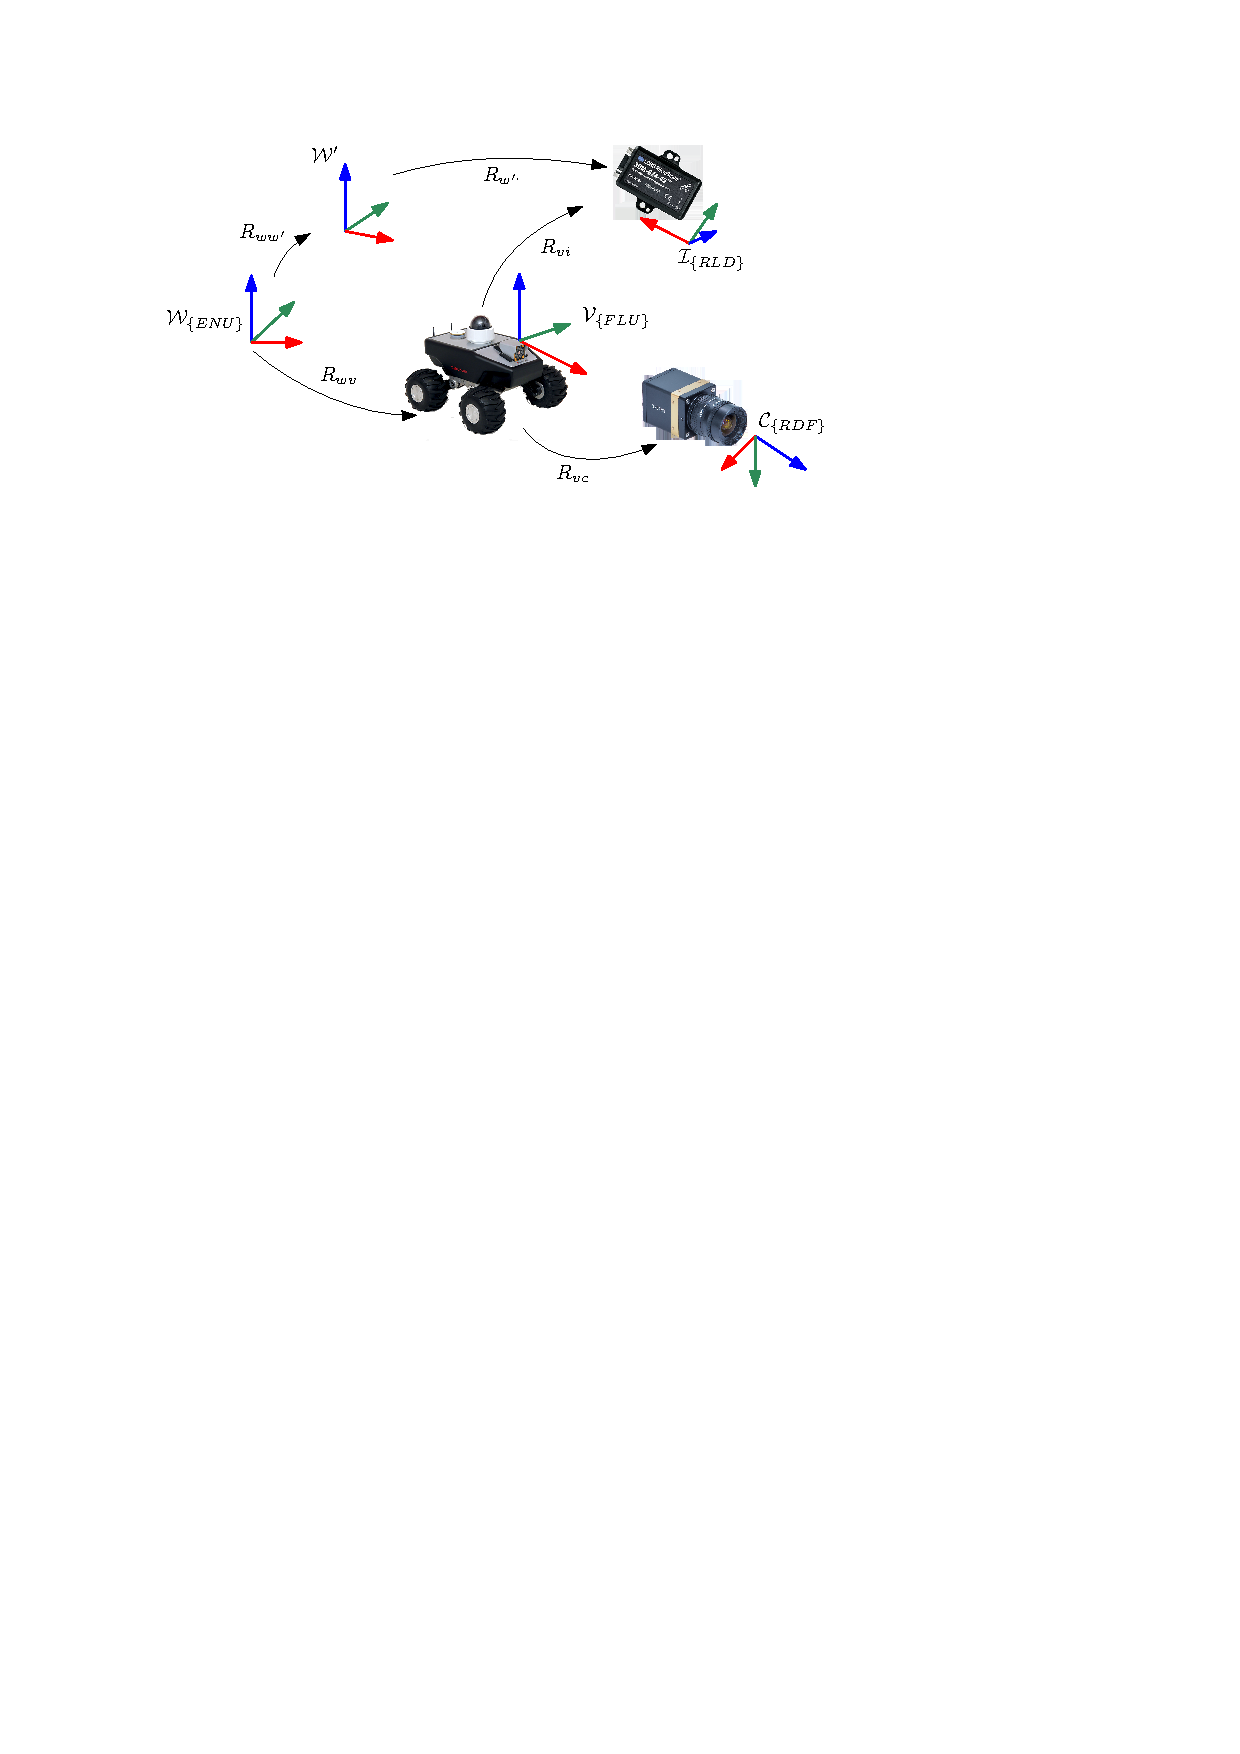
\includegraphics[width=0.5\textwidth]{./content/intro/figures/conventions.pdf}
  \caption{Frame conventions and rotations for attitude estimation of an
    \gls{uav}}
  \label{fig:rotation}
\end{figure}
In Fig.~\ref{fig:rotation} the $\mathcal{W}, \mathcal{W'}, \mathcal{I},
\mathcal{V}, \mathcal{C},$ and $\mathcal{P}$, present the world frame, global
frame of \gls{imu}, \gls{imu} frame, vehicle frame, camera frame, and pixel
frame respectively. Where the rotation from each frame to another is presented
with lowercase alphabet.
In the shown scenario, a vector $v_{p}$ in pixel frame is
expressed in the world frame, $v_{w}$:
\begin{equation}
  \label{eq:vinW}
  v_{w} = R_{wv} \cdot R_{vc} \cdot R_{cp} \cdot v_{p}
\end{equation}
\noindent where the rotation from the camera to the pixel frame $R_{cp}$ is
obtained by camera calibration. The rotation is
defined as the yaw and pitch rotation by the zenith and azimuth angle of the
celestial point ($\theta_c, \phi_c$) as shown in Eq.\,\eqref{eq:Rcp}.
\begin{equation}
  \label{eq:Rcp}
  \begin{split}
  R_{cp}  & =
  \begin{bmatrix}
    \cos\theta_{c}\cos\phi_{c} & -\sin\phi_{c} & \sin\theta_{c}\cos\phi_{c}\\
    \cos\theta_{c}\sin\phi_{c} & \cos\phi_{c} & \sin\theta_{c}\sin\phi_{c}\\
    -\sin\theta_{c} & 0 & \cos\theta_{c}
  \end{bmatrix}
  \\
  & = R_{z_{c}}(\phi_{c})\cdot R_{y_{c}}(\theta_{c})
  \end{split}
\end{equation}

Previously we presented how to express sun position in pixel frame (see
Eq.\,\eqref{eq:sunp}). Indeed this representation is applied to any point from
world frame, ergo:
\begin{equation}
  \label{eq:Rwv}
  \begin{split}
    s_{w} & = R_{wv} \cdot R_{vc} \cdot R_{cp} \cdot
    \begin{bmatrix}
    -\sin\gamma \sin\alpha\\
    \sin\gamma \cos\alpha\\
    \cos\gamma
  \end{bmatrix} = R_{wv} \cdot R_{vc} \cdot v\\
    & R^{T} \cdot s_{w}  = v
  \end{split}
\end{equation}

The above equation shows a direct relationship between the rotation matrix of the vehicle $R$,
the angle of polarization~$\alpha$(that can be measured by the polarimetric camera at one pixel) and the
angle of scattering $\gamma$ for the corresponding pixel. In addition, if $\rho_{lmax}$ is known,
the angle of scattering could be directly obtained by inverting equation~\ref{Eq:cosg} providing a direct relation
between polarization parameters and the rotation of the vehicle.

% Some stuff that emac's colegues use
%%% Local Variables:
%%% mode: late
%%% TeX-master: "../../main.tex"
%%% End: \section{Polarized cues used for attitude estimation}
